\section{Results}
\label{sec:results}


\subsection{RQ1: Minority judgments are treated differently under consensus}

general comparison of majority/minority x consensual/contested
comment score, reply prob/count, engagement



\subsection{RQ2: Minority in consensus - gets lowers scores, more replies/depth/engagement}

from here: we focus on minority in consensual posts only



\subsection{RQ3: The direction of dissent --- accusing versus defending}
\label{subsec:res-direction}

Late Certainty -- dominated by the 'defend' stance

Within the minority of a consensual post, dissent points in one of two moral
directions. \textbf{Accusing} dissent blames an OP the crowd has absolved;
\textbf{defending} dissent absolves an OP the crowd has blamed. The two are
treated differently on every measure we compute, and in the same direction in
both communities (Figure~\ref{fig:direction}).

\textbf{[TODO: report the number of accusing and defending minority comments
per community, and whether the reported scores are means or medians]}

\paragraph{Accusing is penalized more heavily.}
In AITA the average accusing comment scores $-3.2$, against $-2.4$ for
defending. In AITAH, where scores run higher throughout, the gap is wider and
straddles zero: accusing averages $-0.6$ while defending averages $+1.1$. The
ordering is the same in both communities, but AITAH separates the two
directions qualitatively rather than only in degree---a dissenter who defends a
condemned OP ends up with net approval, while one who accuses an absolved OP
does not.

\paragraph{Accusing generates more discussion.}
The engagement measures reverse the sign of the disadvantage. In AITA,
$29.3\%$ of accusing comments draw more than one reply, against $17.2\%$ of
defending comments, and $17.8\%$ seed a subtree deeper than two levels, against
$9.5\%$. AITAH reproduces the pattern at uniformly lower levels: $22.7\%$
versus $12.8\%$ for replies, and $13.2\%$ versus $7.2\%$ for depth. The ratios
are strikingly stable across both communities and both measures: accusing
dissent draws between $1.7$ and $1.9$ times as much discussion as defending
dissent, even as the absolute rates differ by a third between communities.

Sanction and attention therefore do not track a single underlying severity. If
the crowd simply responded more strongly to more objectionable dissent, the two
would move together; instead the direction that is voted down hardest is also
the direction that is answered most. Accusations against a lenient consensus
provoke confrontation, whereas defenses of a condemned OP are more often left
alone.

\begin{figure}[t]
  \centering
  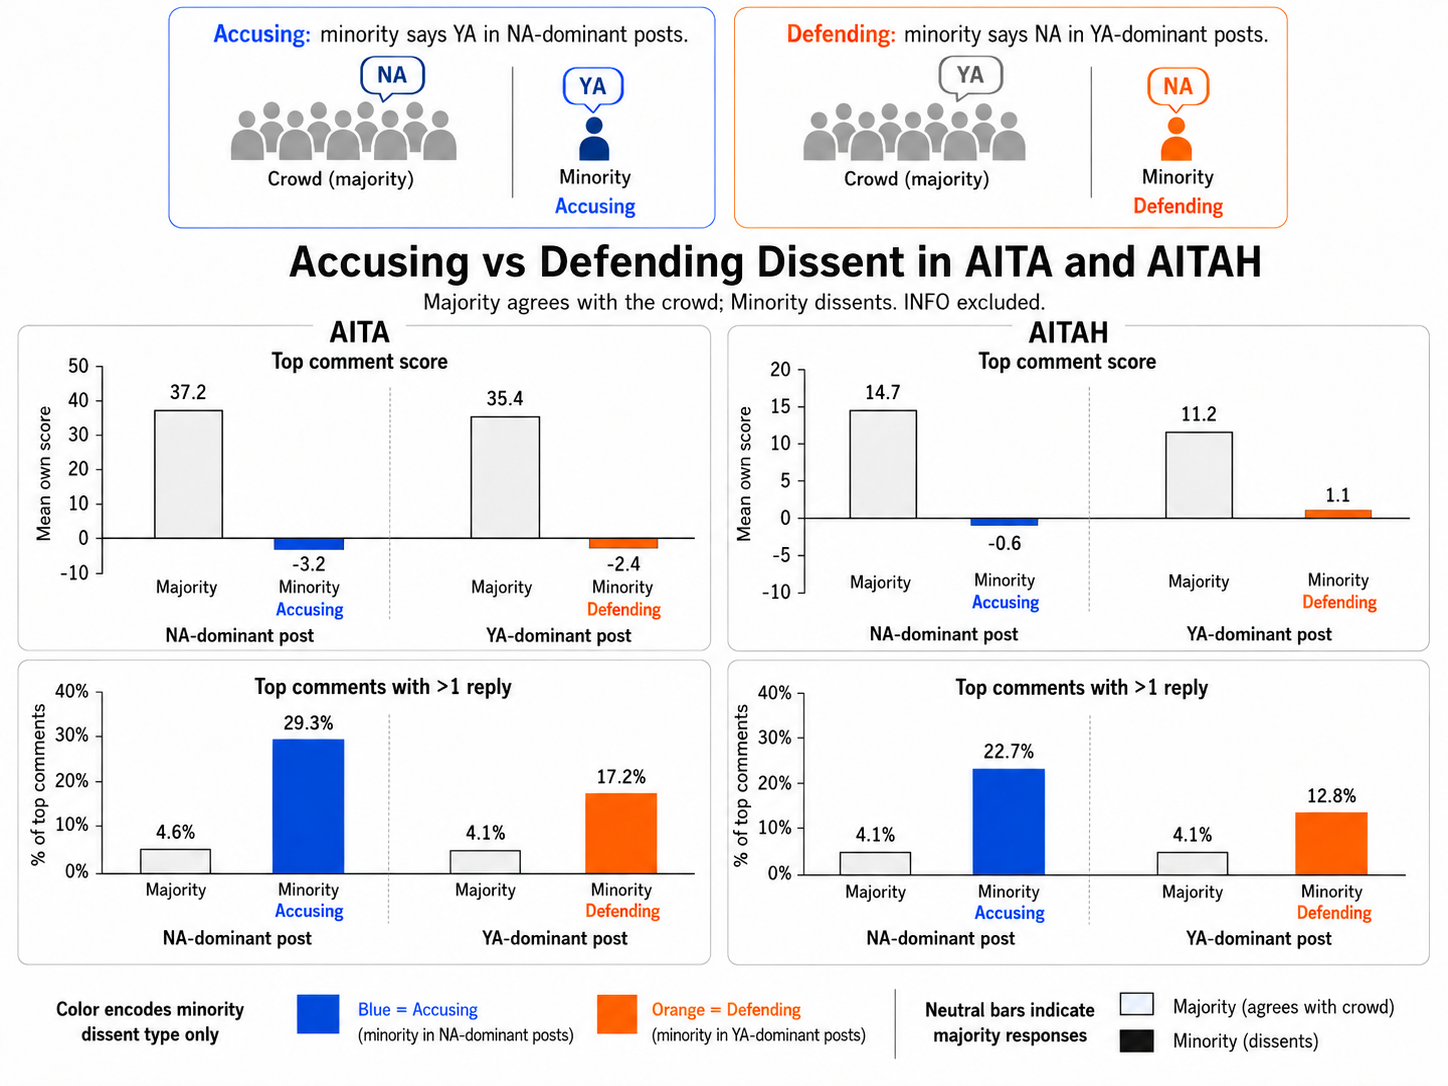
\includegraphics[width=\columnwidth]{figures/direction.png}
  \caption{Accusing versus defending dissent in consensual posts, by community.
  Accusing minority comments score lower than defending ones in both AITA and
  AITAH, yet are $1.7$--$1.9$ times more likely to draw multiple replies and to
  seed reply subtrees deeper than two levels.
  \textbf{[TODO: confirm the figure file name and panel layout]}}
  \label{fig:direction}
\end{figure}



\subsection{RQ4: AITA/AITAH + timeline}
\paragraph{Certainty change over time
18h rule}
Figure~\ref{fig:certainty-time-series} shows the mean certainty expressed by majority- and minority-side comments during the first 25 hours after submission.
Majority-side comments consistently express greater certainty than minority-side comments in both communities. After the 18-hour threshold, minority certainty increases in AITA but decreases temporarily in AITAH.

\paragraph{Minority verdict
ratio over time}


Certainty / share changes over time
18h rule - Formalizing consensus amplifies dissent or not?

\begin{figure}[t]
    \centering
    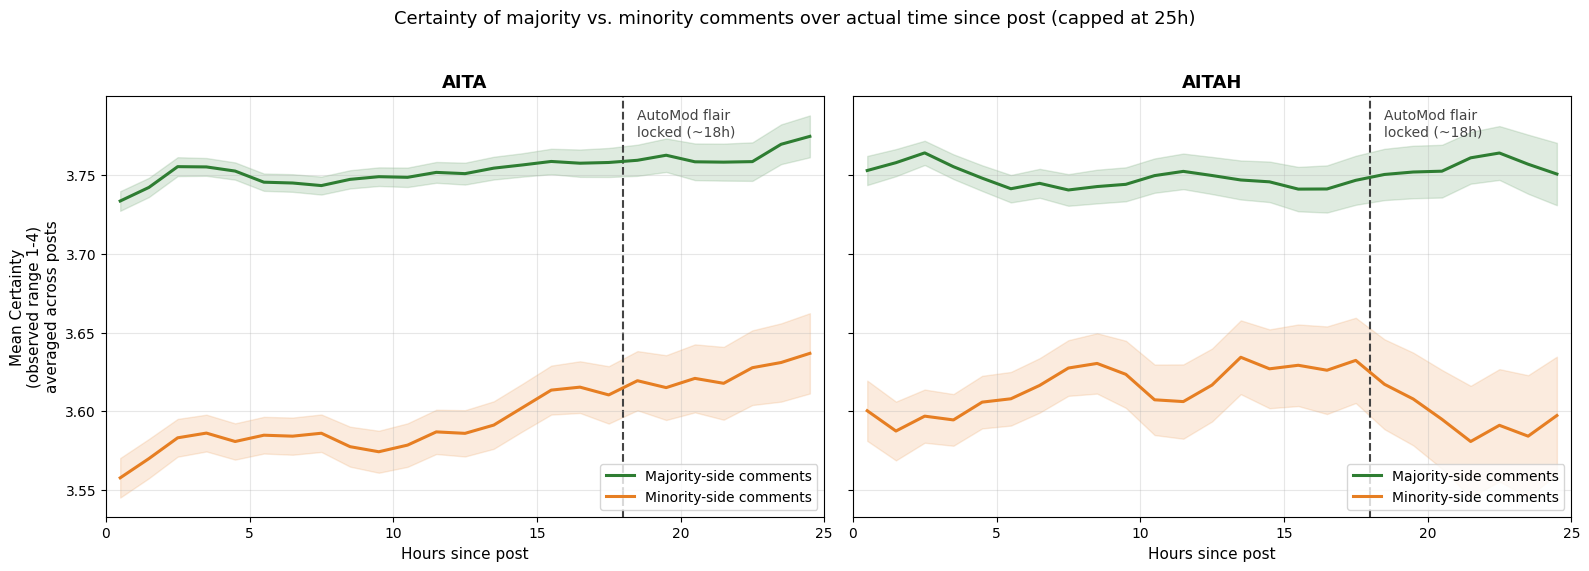
\includegraphics[width=\columnwidth]{figures/time_series_certainty.png}
    \caption{\textbf{Majority voices remain more certain, but the flair-lock
    threshold changes minority certainty only in AITA.}
    Mean certainty of majority- and minority-side comments during the first
    25 hours after submission. The vertical dashed line marks AITA's
    approximately 18-hour AutoModerator verdict-flair lock; it is shown for
    AITAH only as a reference threshold. AITA exhibits a significant increase
    in certainty after this threshold ($p \approx 2 \times 10^{-9}$), whereas
    AITAH does not ($p=.59$).}
    \label{fig:certainty-time-series}
\end{figure}

\subsection{RQ4: AITA/AITAH + shared post in different communities}
\label{subsec:res-duplicates}

community behaviour difference. e.g. minority group is punished more in AITA
